% Options for packages loaded elsewhere
\PassOptionsToPackage{unicode}{hyperref}
\PassOptionsToPackage{hyphens}{url}
%
\documentclass[
]{book}
\usepackage{lmodern}
\usepackage{amssymb,amsmath}
\usepackage{ifxetex,ifluatex}
\ifnum 0\ifxetex 1\fi\ifluatex 1\fi=0 % if pdftex
  \usepackage[T1]{fontenc}
  \usepackage[utf8]{inputenc}
  \usepackage{textcomp} % provide euro and other symbols
\else % if luatex or xetex
  \usepackage{unicode-math}
  \defaultfontfeatures{Scale=MatchLowercase}
  \defaultfontfeatures[\rmfamily]{Ligatures=TeX,Scale=1}
\fi
% Use upquote if available, for straight quotes in verbatim environments
\IfFileExists{upquote.sty}{\usepackage{upquote}}{}
\IfFileExists{microtype.sty}{% use microtype if available
  \usepackage[]{microtype}
  \UseMicrotypeSet[protrusion]{basicmath} % disable protrusion for tt fonts
}{}
\makeatletter
\@ifundefined{KOMAClassName}{% if non-KOMA class
  \IfFileExists{parskip.sty}{%
    \usepackage{parskip}
  }{% else
    \setlength{\parindent}{0pt}
    \setlength{\parskip}{6pt plus 2pt minus 1pt}}
}{% if KOMA class
  \KOMAoptions{parskip=half}}
\makeatother
\usepackage{xcolor}
\IfFileExists{xurl.sty}{\usepackage{xurl}}{} % add URL line breaks if available
\IfFileExists{bookmark.sty}{\usepackage{bookmark}}{\usepackage{hyperref}}
\hypersetup{
  pdftitle={Resultado Final da Disciplina},
  pdfauthor={SIMPLEX (2020.3)},
  hidelinks,
  pdfcreator={LaTeX via pandoc}}
\urlstyle{same} % disable monospaced font for URLs
\usepackage{longtable,booktabs}
% Correct order of tables after \paragraph or \subparagraph
\usepackage{etoolbox}
\makeatletter
\patchcmd\longtable{\par}{\if@noskipsec\mbox{}\fi\par}{}{}
\makeatother
% Allow footnotes in longtable head/foot
\IfFileExists{footnotehyper.sty}{\usepackage{footnotehyper}}{\usepackage{footnote}}
\makesavenoteenv{longtable}
\usepackage{graphicx,grffile}
\makeatletter
\def\maxwidth{\ifdim\Gin@nat@width>\linewidth\linewidth\else\Gin@nat@width\fi}
\def\maxheight{\ifdim\Gin@nat@height>\textheight\textheight\else\Gin@nat@height\fi}
\makeatother
% Scale images if necessary, so that they will not overflow the page
% margins by default, and it is still possible to overwrite the defaults
% using explicit options in \includegraphics[width, height, ...]{}
\setkeys{Gin}{width=\maxwidth,height=\maxheight,keepaspectratio}
% Set default figure placement to htbp
\makeatletter
\def\fps@figure{htbp}
\makeatother
\setlength{\emergencystretch}{3em} % prevent overfull lines
\providecommand{\tightlist}{%
  \setlength{\itemsep}{0pt}\setlength{\parskip}{0pt}}
\setcounter{secnumdepth}{5}
\usepackage{booktabs}
\usepackage{booktabs}
\usepackage{longtable}
\usepackage{array}
\usepackage{multirow}
\usepackage{wrapfig}
\usepackage{float}
\usepackage{colortbl}
\usepackage{pdflscape}
\usepackage{tabu}
\usepackage{threeparttable}
\usepackage{threeparttablex}
\usepackage[normalem]{ulem}
\usepackage{makecell}
\usepackage{xcolor}
\usepackage[]{natbib}
\bibliographystyle{apalike}

\title{Resultado Final da Disciplina}
\author{SIMPLEX (2020.3)}
\date{2020-12-19}

\begin{document}
\maketitle

{
\setcounter{tocdepth}{1}
\tableofcontents
}
\hypertarget{explicando-o-cuxe1lculo-das-notas}{%
\chapter{Explicando o Cálculo das Notas}\label{explicando-o-cuxe1lculo-das-notas}}

Pessoal, fizemos \emph{Lições} (\(N_{_\mathrm{L}}\)), \emph{Atividades Avaliativas} (cuja média denotaremos por \(N_{_\mathrm{AV}}\)), \emph{Provas} (cuja média denotaremos por \(N_{_\mathrm{P}}\)) e \emph{Pontos Extras} (o do \(\LaTeX\) - \(P_{_\mathrm{TeX}}\); e da questão de integral - \(P_{_\mathrm{Int}}\)).

A média final da disciplina (\(M_{_\mathcal{D}}\)) é calculada com a seguinte fórmula:
\[
  M_{_\mathcal{D}} = \frac{3 \cdot N_{_\mathrm{L}} + 3 \cdot  N_{_\mathrm{AV}}  + 4\cdot N_{_\mathrm{P}} }{100} + 
  P_{_\mathrm{TeX}} + P_{_\mathrm{Int}}
\]

Obviamente, a nota máxima alcançada não pode ultrapassar os 10 pontos.

\hypertarget{tabela-das-notas}{%
\chapter{Tabela das Notas}\label{tabela-das-notas}}

A tabela abaixo mostra o resumo até agora.\n
Qualquer discrepância deve ser comunicada imediatamente, visto que tais notas serão postas no \href{https://sistemas.ufrb.edu.br/sigaa/verTelaLogin.do}{SIGAA} ainda hoje (desde quinta eu havia mandado as notas para análise).

Movimente a \emph{barra de rolagem} horizontal até que você veja a \emph{média da disciplina}. Além disso, você pode digitar sua matrícula para individualizar sua análise.

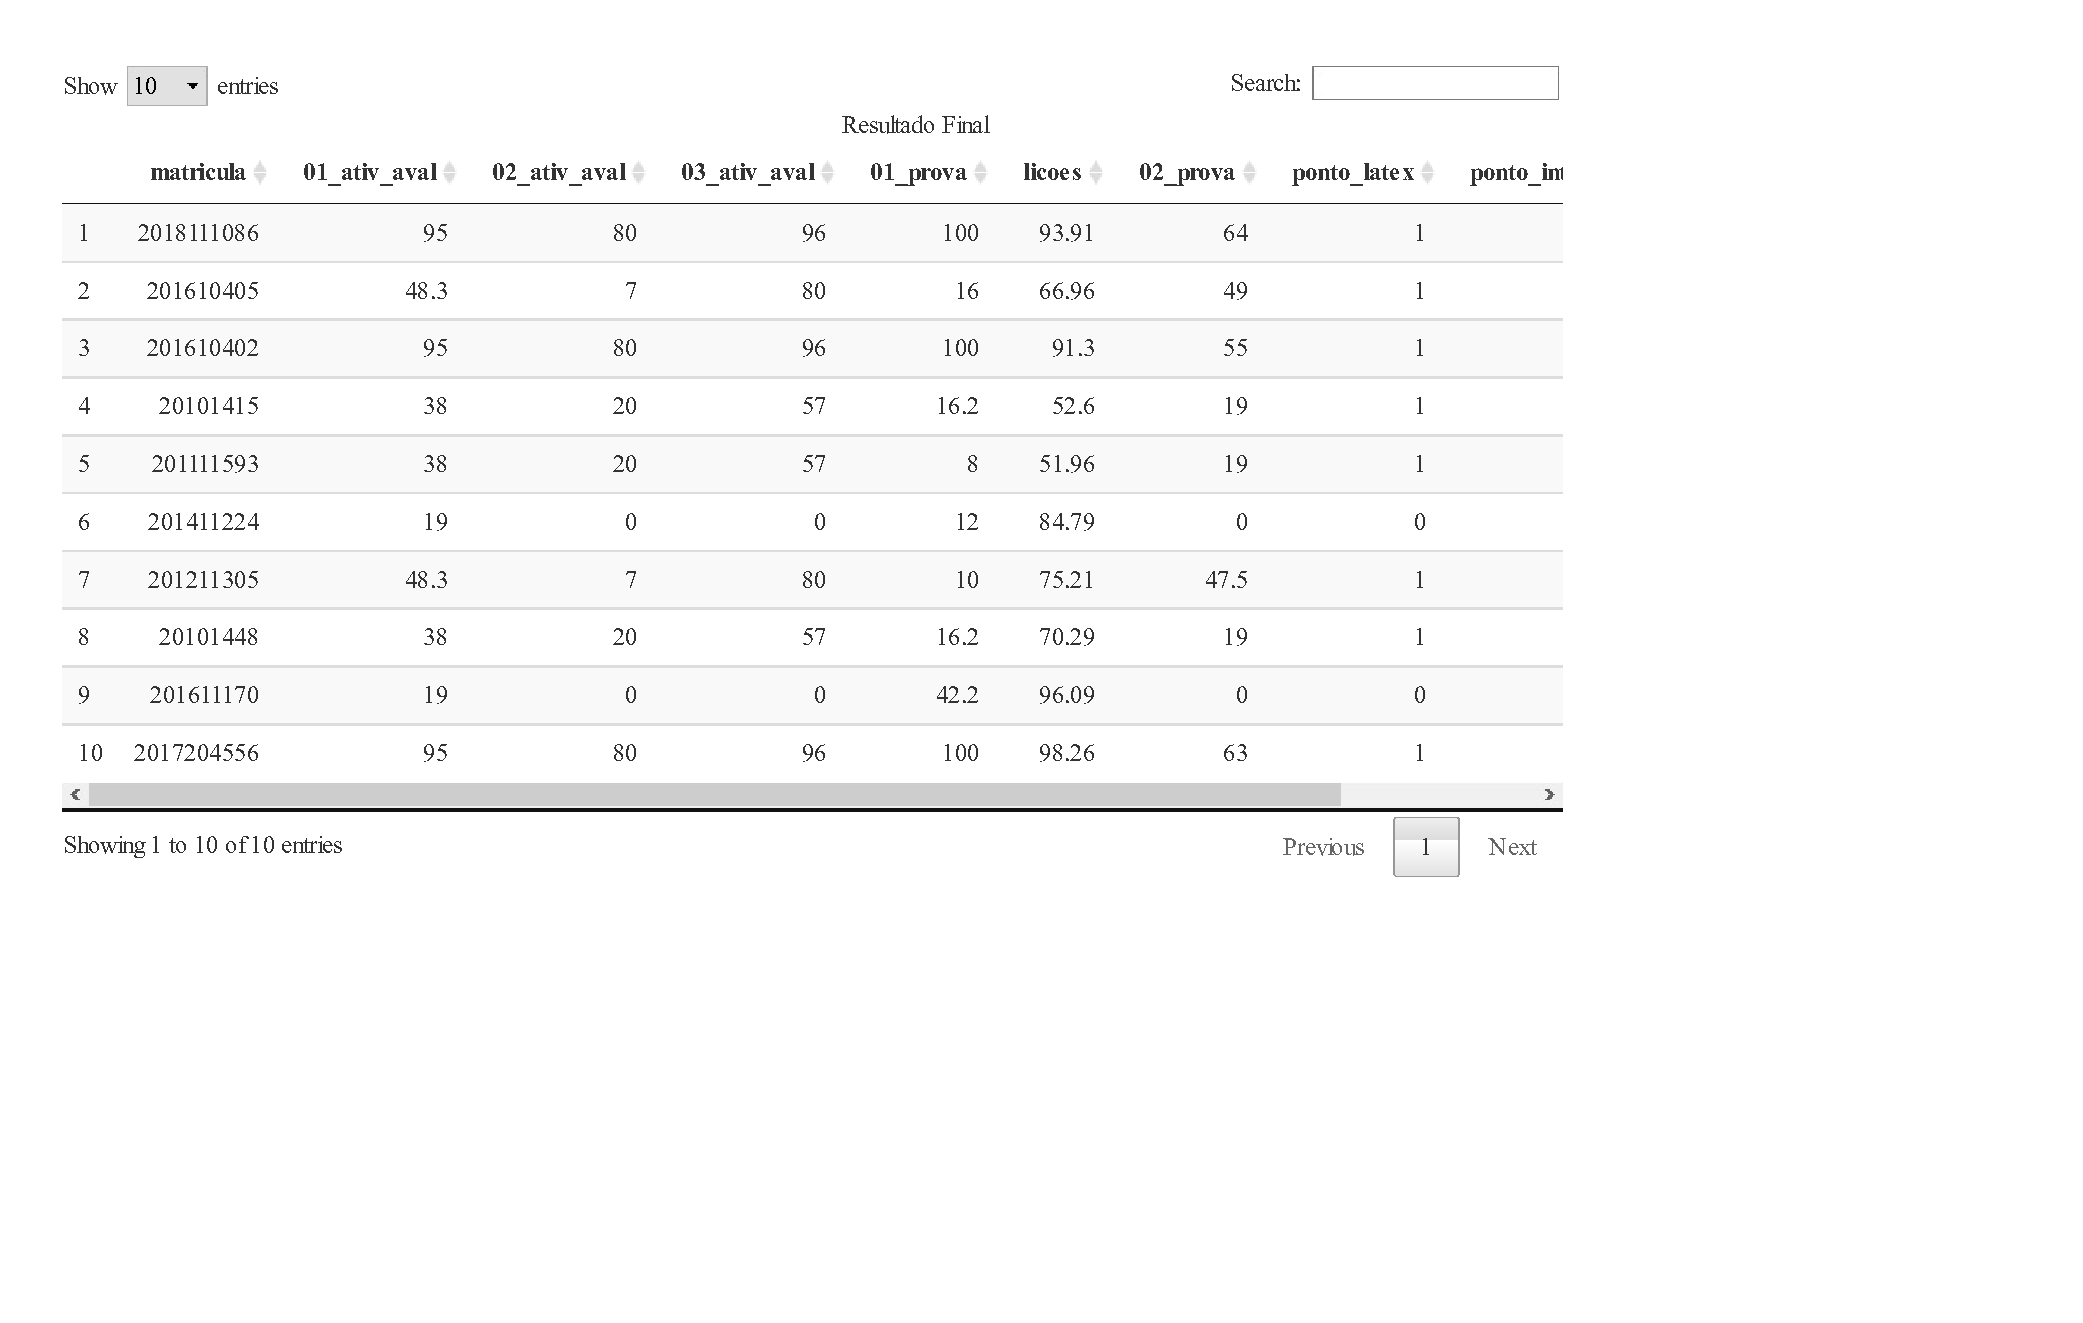
\includegraphics{notas_relatorio_files/figure-latex/unnamed-chunk-1-1.pdf}

\hypertarget{gruxe1fico-boxplot-da-distribuiuxe7uxe3o-das-muxe9dias}{%
\chapter{Gráfico Boxplot da Distribuição das Médias}\label{gruxe1fico-boxplot-da-distribuiuxe7uxe3o-das-muxe9dias}}

Podemos visualizar a distribuição das médias por meio de um gráfico chamado \emph{Bloxplot}.

Boxplots fornecem um bom resumo de uma ou mais variáveis numéricas.

\begin{itemize}
\tightlist
\item
  O segmento de reta horizontal que divide a ``caixa'' em duas partes, representa a \textbf{mediana} dos dados;
\item
  Os segmentos horizontais (ainda da ``caixa''), final e inicial, são, respectivamente, o 3º e o 1º \textbf{quartis}, denotados por \(q_3\) e \(q_1\), respectivamente.
\item
  A diferença entre o 3º e o 1º quartil é denominada \textbf{intervalo interquartil}
  e é denotado por \(IQR\).
\item
  Os segmentos verticais exteriores à caixa são delimitados por \(q_1 - 1.5\cdot IQR\), inferiormente; e por \(q_3 + 1.5\cdot IQR\), superiormente.
\item
  Os pontos fora de tais segmentos verticais são denominados \textbf{outliers} (que não ocorreram nesse semestre).
\end{itemize}

Para construção dos gráficos (que é interativo), excluí os nomes dos discentes que não permaneceram na disciplina até o encerramento da mesma.

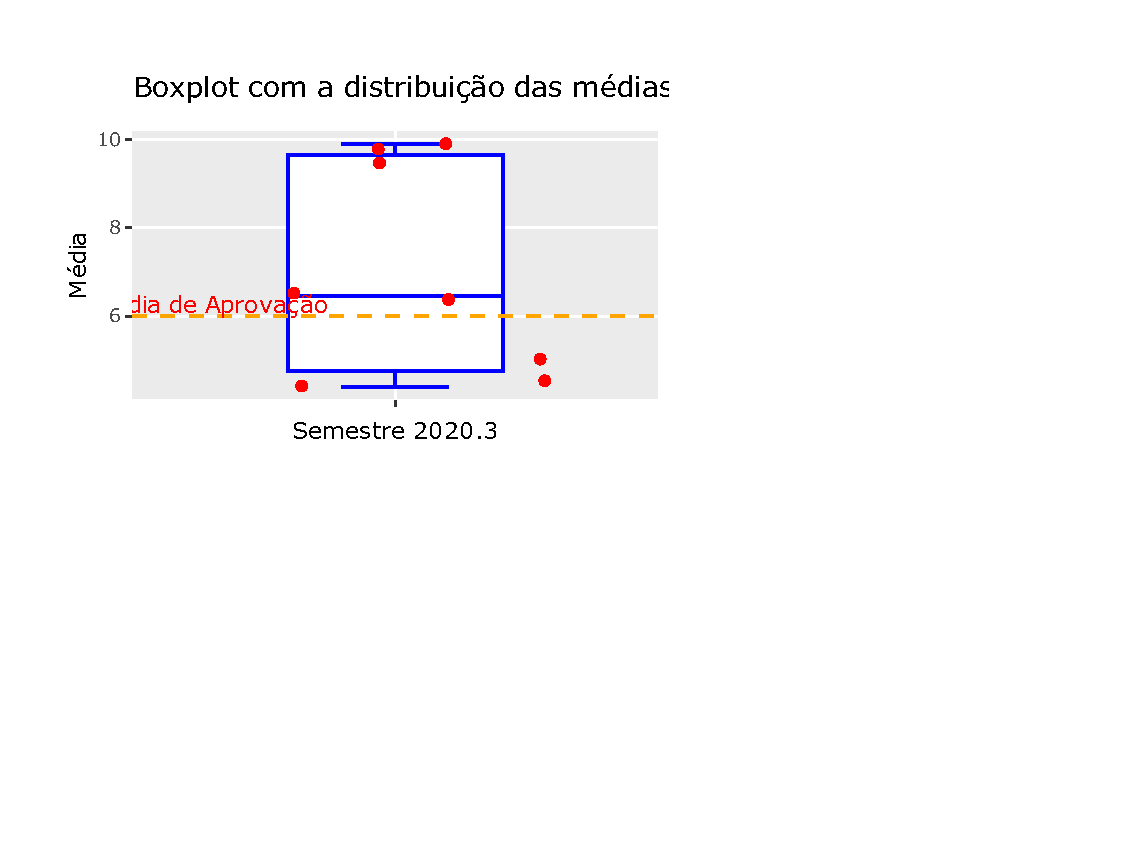
\includegraphics{notas_relatorio_files/figure-latex/unnamed-chunk-2-1.pdf}
No gráfico acima, foi destacada a \emph{Média de Aprovação} da disciplina (que são de 6 pontos).

\hypertarget{palavras-finais}{%
\chapter{Palavras finais}\label{palavras-finais}}

Sei o quanto alguns de vocês se esforçaram durante esse semestre tão atípico.

Nem tudo sai como esperamos, mas desejo que as coisas sejam melhores no próximo semestre.

Boas festas!

  \bibliography{book.bib,packages.bib}

\end{document}
